\begin{frame}
  \frametitle{Fabricated Dataset}
  \begin{table}
    \centering
    \begin{tabular}{p{1.2cm} p{1.8cm} p{1.5cm} p{1.5cm} p{1.5cm} p{1.2cm}}
      \toprule
      Cancer ID & Cancer Label & Population Code & Population & Alpha-3 Code & ASR (World) \\
      \midrule
      1 & Breast Cancer & 1 & 1000000 & ABC & 20.00 \\
      2 & Breast Cancer & 2 & 1500000 & ABC & 21.00 \\
      3 & Breast Cancer & 3 & 2000000 & ABC & 22.00 \\
      4 & Breast Cancer & 4 & 2500000 & DEF & 23.00 \\
      5 & Breast Cancer & 5 & 3000000 & GHI & 24.00 \\
      \bottomrule
    \end{tabular}
    \caption{Sample of Fabricated Dataset}
    \label{tab:fabricated_data}
  \end{table}
  \textit{Note: Only a small sample of the dataset is shown here.}
\end{frame}

\begin{frame}
  \frametitle{Analysis Results}
  \begin{itemize}
    \item Correlation between Population and ASR: -0.0382
    \item Regression slope: -3.862e-07
    \item Y-intercept: 202502.227
    \item Coefficient Standard Deviation: (See full list in output)
  \end{itemize}
\end{frame}

\begin{frame}
  \frametitle{Scatter Plot and Regression Analysis}
  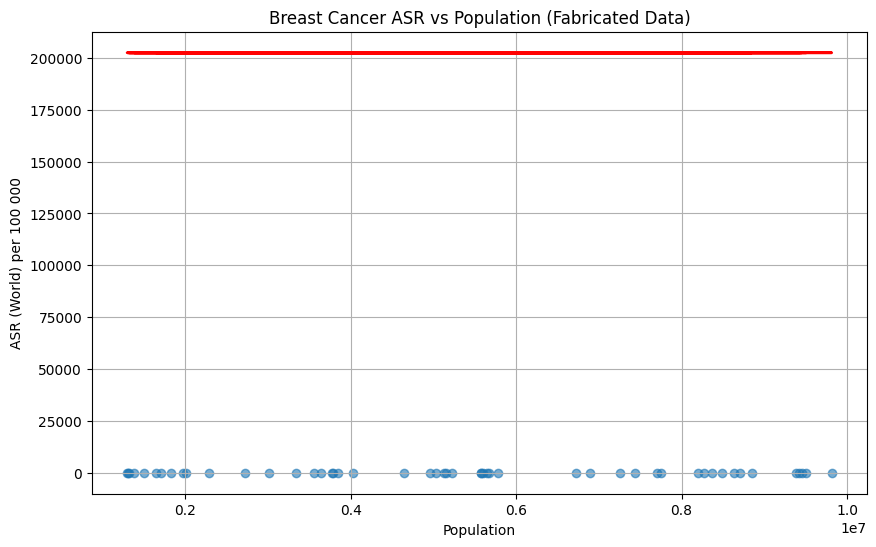
\includegraphics[width=\textwidth]{./images/analysis.png}
  \textit{This plot shows the relationship between Population and ASR, with the regression line.}
\end{frame}

\begin{frame}
  \frametitle{Population vs Cancer Rates Analysis}
  \begin{itemize}
      \item \textbf{Key Findings:}
      \begin{itemize}
          \item No clear connection between country population size and cancer rates
          \item Example: Country A (1M people) vs Country E (3M people) have similar rates
          \item All countries in study show rates between 20-24 cases
      \end{itemize}
      
      \item \textbf{What This Means:}
      \begin{itemize}
          \item Population size doesn't predict cancer rates
          \item Other factors (screening, lifestyle) likely more important
          \item Similar rates across different population sizes
      \end{itemize}
  \end{itemize}
\end{frame}